\chapter{Conclusion}\label{sec:end}
This work addressed the \emph{implementability problem} for Global 
Types, a central concern in the verification of distributed systems. 
After surveying the state of the art, I positioned our contribution 
within an ongoing research effort, bridging well-established 
theoretical foundations with practical tool development.  

On the theoretical side, I introduced the necessary background 
notions-CFSMs, Global Types, MSCs, and communication models-and 
formalized weak realizability. The main contribution was to connect 
the implementability problem to classical undecidability results, in 
particular through a reduction to the Relaxed Post Correspondence 
Problem (RPCP).  

On the practical side, I improved and extended the 
\textsc{ReSCu} tool, used for checking realizability and other semantic 
properties of Symbolic Communicating Machines (SCMs). The input grammar 
was refined for greater usability, and new verification routines were 
implemented, including checks for progress and deadlock-freedom. The tool 
now also generates visual representations of synchronous systems, along 
with illustrative examples. These extensions strengthen 
\textsc{ReSCu} both as a research prototype and as a practical aid for 
automated verification.  

Overall, the contributions span two complementary directions: a refined 
theoretical understanding of implementability, and concrete advances in 
tool support for experimenting with increasingly expressive models. 

\section{Related work}


\chapter{Related work}\label{sec:rel}
This thesis is centred around the study of the \emph{implementability 
problem} for \emph{global types} and MSC-based formal models.  
In this chapter, I review related works addressing this problem, 
both within the same formal framework and in comparable models.  

In particular, this thesis forms part of a broader line of research 
originating from~\cite{di2023partial} and later expanded in 
\cite{di2025realisability}, which aims to develop a general framework 
for communication models. I first present and discuss the results of 
these works, positioning my own contributions in relation to them.  

Subsequently, I analyse recent results by 
Stutz~et~al.~\cite{stutz2024implementability}, who extensively study 
the implementability problem, while also tracing the line of research 
back to early contributions such as Alur~et~al.~\cite{alur2000inference} 
and Lohrey~et~al.~\cite{lohrey2003realizability}.  

Finally, I briefly review related approaches in comparable formal 
models, such as Multiparty Session Types (MPST) and Choreography 
Automata~\cite{barbanera2020choreography}, highlighting similarities 
and differences with respect to the problem addressed in this thesis.

\section{Hierarchy of communication model's semantics}\label{sec:hier}
We defined early some communication semantics of out interest.
Furthermore, \cite{di2023partial} show some other interesting 
semantics. It also introduces a hierarchy of communication
semantics, illustrated in Figure~\ref{fig:coms}. The main objective of
this work was to establish a hierarchy that preserves monotonic
properties: if a property holds for a given communication semantic, it
should also hold for all semantics contained within it. However, it was
shown that this monotonicity only applies to specific properties, such
as \emph{weak-$k$-synchronizability}. In contrast, it does not generally
extend to the implementability problem.

% TODO: rsc =/= sync (messaggi orfani)

\begin{figure}[!ht]
\centering
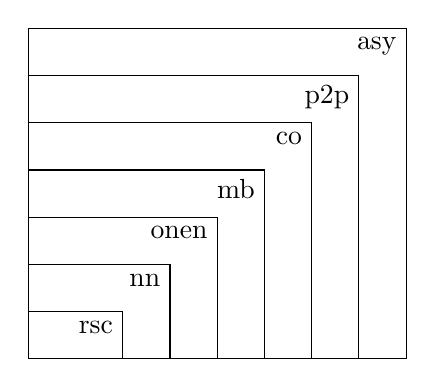
\begin{tikzpicture}[scale=0.6]
  % list of labels in order (from smallest to largest)
%   \def\labels{{rsc,nn,onen,mb,co,p2p,asy}}
  % loop to draw nested squares
  \foreach [count=\i] \lab in {rsc,nn,onen,mb,co,p2p,asy} {
    \draw (0,0) rectangle (\i+1,\i);
    \node[anchor=north east] at (\i+1,\i) {\lab};
  }
\end{tikzpicture}
\caption{Hierarchy of communication model semantics.}
\label{fig:coms}
\end{figure}

% A p2p-MSC is an MSC $M = (E,\to, \lhd, \lambda)$ where, for any two send events $s$ 
% and $s'$ such that $\lambda(s) \in \text{send}(p, q, \_), \lambda(s') in \text{send}(p, q, \_)$, 
% and $s \to^+ s'$, one of the following holds:
% - either $s, s' \in \text{matched}(M)$ with $s \lhd r$ and $s' \lhd r'$ and 
% $r \to^+ r'$,
% - or $s' \in \text{unmatched}(M)$.
% Note that we cannot have two messages $m 1$ and $m 2$, both sent by $p$ to $q$, 
% in that order, such that $m 1$ is unmatched and $m 2$ is matched; unmatched 
% message $m 1$ excludes the reception of any later message.

\paragraph{Peer-to-peer}
In the peer-to-peer communication model $\ppmodel$, every pair of 
processes $(p,q)$ is connected by a dedicated FIFO channel.  
Messages sent by $p$ to $q$ are delivered in the same order in which 
they were issued: if $p$ first sends $m_1$ and then $m_2$, the channel 
guarantees that $m_2$ cannot overtake $m_1$. Concretely:
\begin{itemize}
    \item if $m_1$ is never received, then $m_2$ cannot be received either;
    \item if both are received, then $m_1$ is delivered before $m_2$.
\end{itemize}

\paragraph{Causally ordered}
In the causally ordered (\verb|co|) communication model, messages are delivered 
to a process in accordance with the causal dependencies of their emissions. 
In other words, if there are two messages $m_1$ and $m_2$ with the same recipient, 
such that there exists a causal path from $m_1$ to $m_2$, then $m_1$ must be received 
before $m_2$. This notion of causal ordering was first introduced by Lamport under the 
name ``happened-before'' relation. In Figure~\ref{fig:p2p}, this 
causality is violated: $m_1$ should be received before $m_3$. Causal delivery 
is commonly implemented using Lamport's logical clock algorithm \cite{lamport2019time}.

% An MSC $M = (E, \to, \lhd, \lambda)$ is causally ordered if, for any two send $s$ and 
% $s'$, such that $\lambda(s) \in \text{send}(\_, q, \_), \lambda(s') \in \text{send}(\_, q, \_)$, and 
% $s \leq_{\text{hb}} s'$:
% - either $s, s' \in \text{matched}(M)$ and $r \to^* r'$, with $r$ and $r'$ receive 
% events such that $s \lhd r$ and $s' \lhd r'$.
% - or $s' \in \text{unmatched}(M)$.

% Note that in a \verb|co|-MSC we cannot have two send events $s$ and $s'$ addressed 
% to the same process, such that $s$ is unmatched, $s'$ is matched, and 
% $s \leq_{\text{hb}} s'$.

\paragraph{Mailbox}
In this model, any two messages sent to the same process, regardless of the sender, 
must be received in the same order as they are sent. If a process receives $m_1$ 
before $m_2$, then $m_1$ must have been sent before $m_2$. \verb|mb| coordinates all 
the senders of a single receiver. This model is also called FIFO $n-1$.
In Figure~\ref{fig:mailbox}, an example for this communication model is shown.

\begin{figure}[!ht]
	\centering
	\begin{msc}[draw frame=none, draw head=none, msc keyword=, 
				head height=0px, label distance=0.5ex, 
				foot height=0px, foot distance=0px]{}
		\declinst{p}{p}{}
		\declinst{q}{q}{}
		\declinst{r}{r}{}
		\declinst{s}{s}{}

		\mess[pos=0.1]{$m_4$}{p}{s}[4]
		\nextlevel
		\mess[pos=0.8]{$m_1$}{p}{q}
		\nextlevel
		\mess[pos=0.2]{$m_2$}{r}{q}
		\nextlevel
		\mess[pos=0.8]{$m_3$}{r}{s}
	\end{msc}
	\caption{An example of mailbox semantic.}
	\label{fig:mailbox}
\end{figure}

% An MSC $M = (E, \to, \lhd, \lambda)$ is a \verb|mb|-MSC if it has a linearization 
% $\rightsquigarrow$ where, for any two send events $s$ and $s'$, such 
% that $\lambda (s) \in \text{send}(\_,q,\_), \lambda (s') \in \text{send}(\_,q,\_)$, and 
% $s \rightsquigarrow s'$
% - either $s,s' \in \text{matched}(M)$ and $r \rightsquigarrow r'$, where 
% $s \lhd r$ and $s' \lhd r'$,
% - or $s' \in \text{unmatched}(M)$.

%% TODO: Esistono nella pratica? forse si possono togliere?

\paragraph{FIFO 1-n}
This model (\verb|onen|) is the dual of \verb|mb|, it coordinates a sender with all the 
receivers. Any two messages sent by a process must be received in the same 
order as they are sent. These two messages might be received by different 
processes and the two receive events might be concurrent.

% An MSC $M = (E, \to, \lhd, \lambda)$ is a \verb|onen|-MSC if it has a linearization 
% $\rightsquigarrow$ where, for any two send events $s$ and $s'$, such 
% that $\lambda (s) \in \text{send}(p,\_,\_), \lambda (s') \in \text{send}(p,\_,\_)$ and 
% $s \to^+ s'$ (which implies $s \rightsquigarrow s'$)
% - either $s,s' \in \text{matched}(M)$ and $r \rightsquigarrow r'$, with 
% $r$ and $r'$ receive events such that $s \lhd r$ and $s' \lhd r'$,
% - or $s' \in \text{unmatched}(M)$.

\paragraph{FIFO n-n}
In this model (\verb|nn|), messages are globally ordered and delivered according to 
their emission order. Any two messages must be received in the same order 
as they are sent. These two messages might be sent or receives by any process 
and the two send or receive events might be concurrent. The FIFO \verb|n-n| 
coordinates all the senders with all the receivers.

% An MSC $M = (E, \to, \lhd, \lambda)$ is a \verb|nn|-MSC if it has a linearization 
% $\rightsquigarrow$ where, for any two send events $s$ and $s'$, such 
% that $s \rightsquigarrow s'$
% - either $s, s' \in \text{matched}(M)$ and $r \rightsquigarrow r'$, with $r$ 
% and $r'$ receive events such that $s \lhd r$ and $s' \lhd r'$,
% - or $s' \in \text{unmatched}(M)$.
\paragraph{RSC}
Figure~\ref{fig:coms} shows \verb|rsc| as the last block of the hierarchy.
\verb|rsc| stands for \emph{Realisable in Synchronous Communication}, therefore, 
is comparable to our definition of $\synchmodel$ model, but there are 
some differences. For example, it does not accept \emph{orphan messages}, 
which are instead accepted for the defintion of this thesis.

\section{Realisability for MSCs}

For finite sets of MSCs, weakly realisability as defined in 
\cite{alur2005realizability} is \verb|coNP|-complete and safe 
realisability is shown to be decidable in \verb|P|-time~\cite{alur2005realizability}.
The problem was subsequently studied for infinite MSC languages, defined 
as MSC-Graphs (MSGs). For bounded MSGs, safe realisability 
remains decidable, but weak realisability 
is undecidable~\cite{alur2005realizability}. Extensions of these results to non-FIFO 
semantics were investigated in~\cite{morin2002recognizable}, corresponding 
to bag semantics under peer-to-peer communication. 
Later, Lohrey proved that in the general case, safe realisability 
is undecidable~\cite{lohrey2003realizability}, though it is decidable (and 
\verb|EXPSPACE|-complete) for MSGs. %for globally cooperative MSGs.
Most positive results assume bounded channels, but \cite{bollig2025high} introduces 
a new class of HMSCs that allows unbounded channels while maintaining implementability.
A summary of the main complexity results is given in Table~\ref{tab:realisability}.

\begin{table}[!ht]
	\centering
	\begin{tabular}{|l|c|c|c|}
		\hline
		& \textbf{Finite set} & \textbf{Bounded graphs} & \textbf{Unbounded} \\
		\hline
		\textbf{Weak} & \verb|coNp|-complete & undecidable & undecidable \\
		\hline
		\textbf{Safe} & P-time & \verb|EXPSPACE|-complete & undecidable \\
		\hline
	\end{tabular}
	\caption{Summary of results on realisability.}
	\label{tab:realisability}
\end{table}

\section{Realisability for MPST}

Recent work has focused on strengthening the connection between MPST 
and automata-theoretic formalisms. Stutz and Zufferey 
showed that implementability is decidable by encoding global types 
into HMSCs that are globally cooperative~\cite{stutz2022comparing,stutz2023asynchronous}. 
Building on this, Li et al.~\cite{li2023complete} proposed a complete 
projection function for MPST, guaranteeing that every implementable 
global type admits a correct distributed implementation.

Stutz’s thesis~\cite{stutz2024implementability} connects MPST to 
High-level MSCs (HMSCs), introducing a generalized projection operator 
for sender-driven choice where a sender may branch towards different 
receivers. This captures patterns beyond classical MPST projection.  
He also proves that while syntactic projection is incomplete, 
an automata-theoretic encoding into HMSCs yields decidability for 
sender-driven choice, with implementability shown to be in 
\verb|PSPACE|-the first precise complexity bound for this fragment.

\section{Choreographies}
Choreographies \cite{montesi2014choreographic} are another formalism to describe  
distributed communication protocols. Unlike MSCs or MPST, which focus either on 
trace-based semantics or type systems, choreographies emphasize the 
global specification of interactions as a high-level description of the 
intended message exchanges. Similarly to MPST, their goal is to ensure that
a distributed  implementation can be derived in which each participant 
follows a local behaviour consistent with the global description, called
respectively \emph{local} and \emph{global-view}. This setting naturally 
connects to the realisability problem, since the key question is whether 
a choreography can be faithfully implemented by a system of local 
processes. In choreographies, the local-view is called \textbf{End-Point Projection} (EPP),
and it is derived throughout a projection operation from the global-view.
The \emph{knowledge of choice} problem is similar to the implementability one,
and explored also in choreographies,
but it was first introduced by Castagna et al.~\cite{castagna2012global}.
% https://www.fabriziomontesi.com/bliki/KnowledgeOfChoice#CHY12
% TODO: Continuare menzionando che i chor automata sono simili alla nostra 
% definizione di global type

\section{Other works}
%citare il paper di Emilio su pomsets
Stutz et al.~\cite{stutz2025automata} proposed \emph{Protocol State Machines} 
(PSMs), an automata-based formalism subsuming both MPST and HMSCs. 
PSMs show that many syntactic restrictions of global types are not 
true expressivity limits. Yet, the implementability problem for PSMs 
with unrestricted mixed choice remains undecidable, resolving the 
open question that mixed-choice global types are undecidable in general.  

In summary, projectability is well understood for sender-driven choice, 
where decidability and complexity bounds are established, but moving 
towards mixed choice inevitably leads to undecidability. Automata-based 
techniques such as HMSCs and PSMs provide the most powerful tools for 
extending the theory while preserving decidability in restricted cases.

\section{Future Work}
Future directions include extending the theoretical results beyond weak 
realizability toward a decidability result of \emph{safe realizability} 
(therefore, including deadlock-freedom) for 
Global Types, building on the techniques developed here and extending
an existing proof made by Lohrey, et al. \cite{lohrey2003realizability}.
On the practical side, a natural goal is to further enhance \textsc{ReSCu} to  
support these results, ultimately aiming for a complete algorithm to decide 
implementability for restricted classes of Global Types. This would 
enable systematic benchmarking against existing methods and real-world 
protocols.